\documentclass[tikz,border=10pt]{standalone}
\usepackage{tkz-euclide} % 增强几何绘图功能

\begin{document}
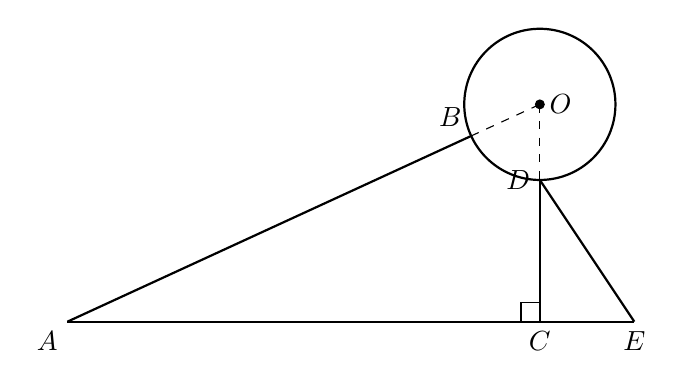
\begin{tikzpicture}[scale=1.2, >=stealth]
    % 1. 定义核心坐标点
    \coordinate (A) at (0, 0);
    \coordinate (C) at (5, 0);
    \coordinate (E) at (6, 0);
    \coordinate (D) at (5, 1.5);
    \coordinate (O) at (5, 2.3); % 圆心位置在D上方
    
    % 计算点B：B在直线AO上，且在圆O上
    % 圆的半径为 r = OD = (2.3 - 1.5) = 0.8
    \def\radius{0.8}
    \path (O) +({atan2(0-2.3, 0-5)}:\radius) coordinate (B);

    % 2. 绘制主要实线部分
    \draw[thick] (A) -- (E);          % 底边 AE
    \draw[thick] (C) -- (D);          % 垂线 CD
    \draw[thick] (D) -- (E);          % 斜边 DE
    \draw[thick] (A) -- (B);          % 线段 AB
    
    % 3. 绘制圆 O
    \draw[thick] (O) circle (\radius);
    \fill (O) circle (1.5pt);         % 圆心实心点

    % 4. 绘制辅助虚线
    \draw[dashed] (B) -- (O);         % 半径 OB
    \draw[dashed] (O) -- (D);         % 半径 OD (垂直向)

    % 5. 绘制直角符号
    \draw (4.8, 0) -- (4.8, 0.2) -- (5, 0.2);

    % 6. 标注文本标签
    \node[below left] at (A) {$A$};
    \node[below]      at (C) {$C$};
    \node[below]      at (E) {$E$};
    \node[left]       at (D) {$D$};
    \node[above left] at (B) {$B$};
    \node[right]      at (O) {$O$};

\end{tikzpicture}
\end{document}